
%!TEX encoding = UTF-8 Unicode
% !TeX spellcheck = en_GB


%%%%%%%%%%%%%%%%%%
%\appendix
%%%%%%%%%%%%%%%%%%%

%%%%%%%%%%%%%%%%%%
\chapter{Alternative simplified models for the flavour anomalies}
\label{app:EW}
%%%%%%%%%%%%%%%%%%
Working under the PDD ansatz, it is possible to consider that the model would couple to the electron instead of the muon. Not much would change in terms of the particle content of this model, except for opposite charge assignment to get correct signs for the Wilson coefficients of $\mathcal O^{Lu}$ and $\mathcal O_{\phi L}^{(1)}$ seen in the right panel off~\autoref{fig:2D_correlations}. The electron and top partners need opposite $X$ charges in this case.
A final comment is needed for the electron scenario reported in~\autoref{fig:2D_correlations_e}, that involves opposite signs for the Wilson coefficients of $\mathcal O^{Lu}$ and $\mathcal O_{\phi L}^{(1)}$ discussed so far. For the former, it should be noted that the sign highlighted in the matching in eq.~\eqref{eq:CLu_Zprime} follows from having assumed the same sign for the charge of the vector-like top and muon partners under $U(1)_{X}$. For what concerns the generation of $C_{\phi L}^{(1)} \ ^{11} < 0 $, according to eq.~\eqref{eq:matching_CHL} one needs to correlate once again the contribution stemming from $S_{0}$, or from $S_{1}$, with the effect coming from a $SU(2)_{L}$ triplet, that now needs to be identified with $T_{1}$, namely the triplet of hypercharge $Y=1$.
\begin{figure}[htpb!]
	\centering
	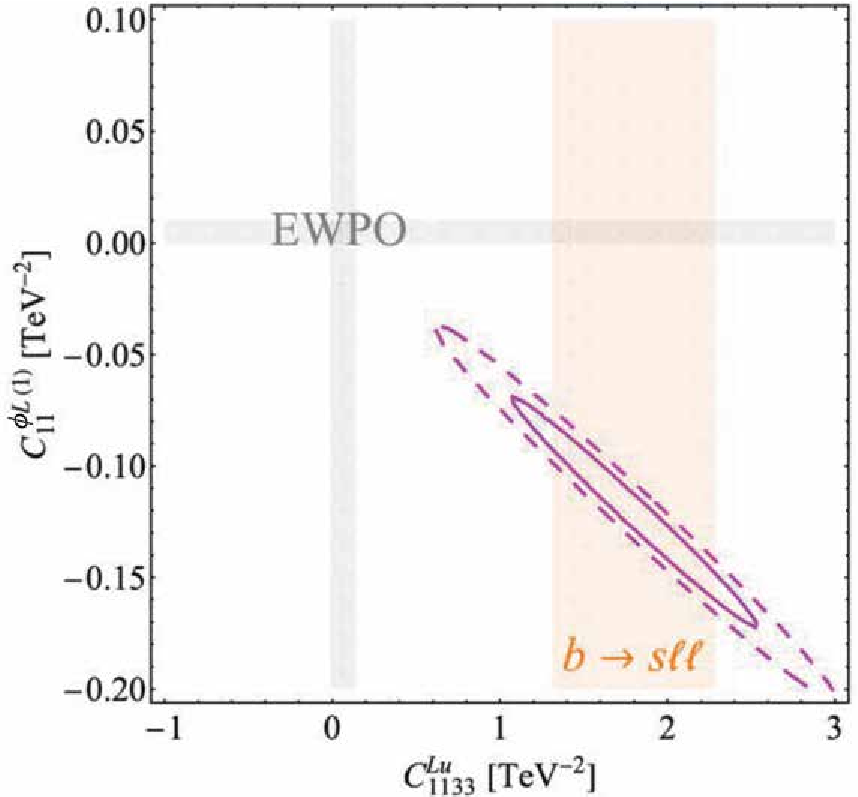
\includegraphics[width=0.5\textwidth]{figures/CHL_CLu_e.pdf}
	\caption{ A minimal solution for the flavour anomalies within SMEFT while respecting EWPO for the four-fermion operators involving the electron. EWPO fits are the grey regions, while the $b \to s\ell \ell$ measurements fits with PDD ansatz are highlighted by the orange bands. The combined fit's 1 and 2$\sigma$ contours are magenta coloured. This plot has been published in~\cite{Alasfar:2020mne}.  } 
	\label{fig:2D_correlations_e}
\end{figure}
Eventually, we wish also to comment on the possible role of the $\mathcal O_{eu}$ operator, so far neglected in this discussion, but of potential relevance more in general. As mentioned earlier, the presence of $\mathcal O_{eu}$ would be particularly needed in the case where hadronic corrections entering in the amplitude of $B \to K^* \ell \ell $ would be of the size originally estimated in~\cite{Khodjamirian:2010vf}. 
In that case, a solution to flavour anomalies would be preferred in the muonic channel with NP Wilson coefficient $C_{eu}^{2233}$ also substantially deviating from 0. Then, one would need to involve also the operator $C_{\phi e}^{22}$ to relieve possible tensions with EW precision. In a general picture, the required NP effects from $ \mathcal O_{\phi e}^{11,22}$ can be obtained by integrating out heavy vector-like $SU(2)_{L}$ leptonic doublets.